\section{Park, Kim - Quadruped Bounding Control with Variable Duty Cycle via Vertical Impulse Scaling - 2014}


\subsection*{Summary}
The strategy used by Park et al. consists in predefinig a given GRF profile parametrized by two Bezier curves. The overall force profile is normalized in such a way that the total energy given to the system in one stance period is equal to the work carried out by gravity during the flight phase $T$.
The relation is thus:

\begin{equation}
2 \alpha c T_{stance} = m g T
\end{equation}
where:
\begin{itemize}
\item c = normalizing factor
\item $\alpha$ = scaling factor
\end{itemize}
This model is completely stiff and the stance time decreases with the incrementation of the forward speed. The forward and vertical speeds are considered as decoupled though.\\
The next step consists in finding stable limit cycles; this is done by mean of the Poincarè Map: the system is linearized around a huge number of fixed points (varying both the Duty cycle and the stiffness of the PD controller) and the largest eigenvalue for each combination is plotted in a graph. In this graph only those eigenvalues which are smaller than 1 are considered as a stable solution. The final choice is made for the values of Duty cycle and stiffness which ensure the largest stability margin.
\begin{figure}[h]
  \centering
  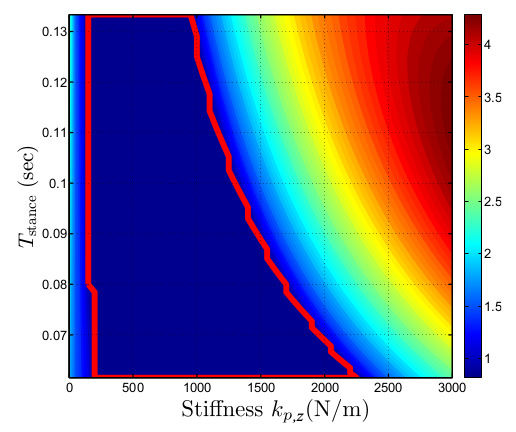
\includegraphics[width=100mm]{PoincarèMap.png}
  \caption{Poincarè Map to evaluate a stable solution}
  \label{InftyCap}
\end{figure}
\subsection*{Key Points / Takeaways}
\begin{itemize}
\item assumed values:
\begin{itemize}
\item $T_{swing} = 220$ ms;
\item $T_{air} = 43.5$ ms;
\item $T_{stance} = 66:133$ ms;
\item $T = T_{stance} + T_{swing}$
\item Duty cycle $D = 0.223:0.377$
\end{itemize}
\item horizontal and vertical speeds are considered as decoupled
\end{itemize}


\subsection*{Weak Points}

\begin{itemize}
\item In this paper there is no consideration of the landing and take off angle of the legs (angle of attack/"incidenza"). The GRF are computed using the trunk model only and massless legs. Therefore the dynamics of the legs is ignored and the compliance is not exploited.
\end{itemize}
\subsection*{Ideas} 
\begin{enumerate}
\item What about minimizing the stiffness of the SLIP model is such a way to damp the force peaks as much as possible??
\end{enumerate}
